\documentclass{article}
\usepackage{graphicx} % Required for inserting images
\usepackage{tikz}
\usetikzlibrary{automata, positioning}

\title{AFD}
\author{Adrian Sandoval Huamani}
\date{July 2023}

\begin{document}

\maketitle

\section{Basics}

\subsection{Definiciones}

\begin{itemize}
    \item Un AFD es una $5$-tupla $(Q,\sum,\delta,q_0,F)$ 
\end{itemize}

\section{Diagrams}

\centering
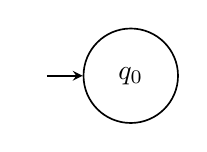
\begin{tikzpicture}[->, >=stealth, auto, node distance=2.9cm, semithick]
  % Definir los estados
  \node[state, initial, initial text={}] (q0) [minimum size=1.2cm] {$q_0$};
  % \node[state, accepting, right of=q0] (q1) [minimum size=1.2cm] {$q_1$};

  % Dibujar las transiciones
  % \draw (q0) edge[loop above] node{0} (q0);
  % \draw (q0) edge[bend left] node{1} (q1);
  % \draw (q1) edge[loop above] node{1} (q1);
  % \draw (q1) edge[bend left] node{0} (q0);
\end{tikzpicture}


\end{document}
